\documentclass[12pt,letterpaper]{article}
\usepackage{graphicx,textcomp}
\usepackage{natbib}
\usepackage{setspace}
\usepackage{fullpage}
\usepackage{color}
\usepackage[reqno]{amsmath}
\usepackage{amsthm}
\usepackage{fancyvrb}
\usepackage{amssymb,enumerate}
\usepackage[all]{xy}
\usepackage{endnotes}
\usepackage{lscape}
\newtheorem{com}{Comment}
\usepackage{float}
\usepackage{hyperref}
\newtheorem{lem} {Lemma}
\newtheorem{prop}{Proposition}
\newtheorem{thm}{Theorem}
\newtheorem{defn}{Definition}
\newtheorem{cor}{Corollary}
\newtheorem{obs}{Observation}
\usepackage[compact]{titlesec}
\usepackage{dcolumn}
\usepackage{tikz}
\usetikzlibrary{arrows}
\usepackage{multirow}
\usepackage{xcolor}
\newcolumntype{.}{D{.}{.}{-1}}
\newcolumntype{d}[1]{D{.}{.}{#1}}
\definecolor{light-gray}{gray}{0.65}
\usepackage{url}
\usepackage{listings}
\usepackage{color}

\definecolor{codegreen}{rgb}{0,0.6,0}
\definecolor{codegray}{rgb}{0.5,0.5,0.5}
\definecolor{codepurple}{rgb}{0.58,0,0.82}
\definecolor{backcolour}{rgb}{0.95,0.95,0.92}

\lstdefinestyle{mystyle}{
	backgroundcolor=\color{backcolour},   
	commentstyle=\color{codegreen},
	keywordstyle=\color{magenta},
	numberstyle=\tiny\color{codegray},
	stringstyle=\color{codepurple},
	basicstyle=\footnotesize,
	breakatwhitespace=false,         
	breaklines=true,                 
	captionpos=b,                    
	keepspaces=true,                 
	numbers=left,                    
	numbersep=5pt,                  
	showspaces=false,                
	showstringspaces=false,
	showtabs=false,                  
	tabsize=2
}
\lstset{style=mystyle}
\newcommand{\Sref}[1]{Section~\ref{#1}}
\newtheorem{hyp}{Hypothesis}

\title{Problem Set 3}
\date{Due: February 17, 2020}
\author{QTM 200: Applied Regression Analysis}

\begin{document}
	\maketitle
	
	\section*{Instructions}
	\begin{itemize}
		\item Please show your work! You may lose points by simply writing in the answer. If the problem requires you to execute commands in \texttt{R}, please include the code you used to get your answers. Please also include the \texttt{.R} file that contains your code. If you are not sure if work needs to be shown for a particular problem, please ask.
		\item Your homework should be submitted electronically on the course GitHub page in \texttt{.pdf} form.
		\item This problem set is due at the beginning of class on Monday, February 17, 2020. No late assignments will be accepted.
		\item Total available points for this homework is 100.
	\end{itemize}
	
		\vspace{.25cm}
	
\noindent In this problem set, you will run several regressions and create an add variable plot (see the lecture slides) in \texttt{R} using the \texttt{incumbents\_subset.csv} dataset. Include all of your code.

	\vspace{.5cm}
\section*{Question 1 (20 points)}
\vspace{.25cm}
\noindent We are interested in knowing how the difference in campaign spending between incumbent and challenger affects the incumbent's vote share. 
	\begin{enumerate}
		\item Run a regression where the outcome variable is \texttt{voteshare} and the explanatory variable is \texttt{difflog}.\\	
		I first load the dataset into R and rename it as $"$incum$"$. Then I run the regression with X variable as difflog and Y variable as voteshare. I then check the estimateed coefficients of the model using \texttt{summary()}.\\
		\lstinputlisting[language=R, firstline=17, lastline=21]{PS3_answer.R}  	
		\begin{footnotesize}
		
		\begin{verbatim}
		Coefficients:
		Estimate Std. Error t value Pr(>|t|)    
		(Intercept) 0.579031   0.002251  257.19   <2e-16 ***
		difflog     0.041666   0.000968   43.04   <2e-16 ***
		---
		Signif. codes:  0 ‘***’ 0.001 ‘**’ 0.01 ‘*’ 0.05 ‘.’ 0.1 ‘ ’ 1
		
		Residual standard error: 0.07867 on 3191 degrees of freedom
		Multiple R-squared:  0.3673,	Adjusted R-squared:  0.3671 
		F-statistic:  1853 on 1 and 3191 DF,  p-value: < 2.2e-16
		\end{verbatim}
	\end{footnotesize}
		
		\item Make a scatterplot of the two variables and add the regression line. 	
		\begin{figure}[h!]\centering
		\caption{\footnotesize Scatterplot of \texttt{voteshre} and \texttt{difflog}.
		}\vspace{-1cm}
		\label{fig:plot1}
		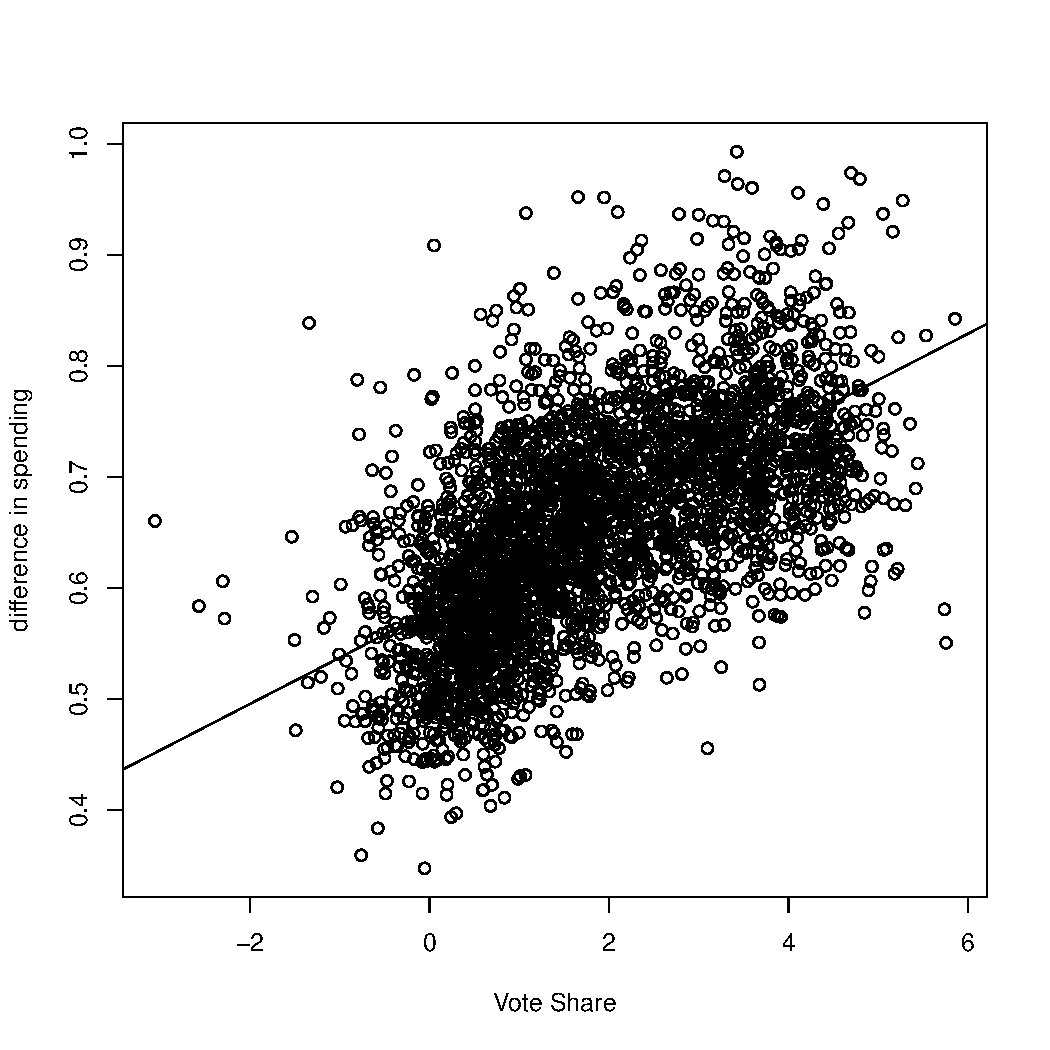
\includegraphics[width=.75\textwidth]{plot1.pdf}
	\end{figure}
	\vspace{.25cm}
		\item Save the residuals of the model in a separate object.	
		\lstinputlisting[language=R, firstline=31, lastline=32]{PS3_answer.R}  
		\item Write the prediction equation.\vspace{.25cm}

		The simple linear prediction equation is $\hat{Y_{i}}={\beta_{0}}+{\beta_{1}}*X_i$.\\ I use the coefficients from the previous question to find ${\beta_{0}}$, which is the $Y-intercept$ when $X=0$, and ${\beta_{0}}$, which is the estimated slope.
		\lstinputlisting[language=R, firstline=36, lastline=37]{PS3_answer.R}
		The prediction equation is $\hat{Y_{i}}=0.579+0.042*X_i$.\\
	\end{enumerate}
	
\newpage

\section*{Question 2 (20 points)}
\noindent We are interested in knowing how the difference between incumbent and challenger's spending and the vote share of the presidential candidate of the incumbent's party are related.	\vspace{.25cm}
	\begin{enumerate}
		\item Run a regression where the outcome variable is \texttt{presvote} and the explanatory variable is \texttt{difflog}.\\
		I run the regression with X variable as \texttt{difflog} and Y variable as \texttt{presvote}. I then check the estimateed coefficients of the model using \texttt{summary()}.\\
		\lstinputlisting[language=R, firstline=47, lastline=50]{PS3_answer.R}
		\begin{footnotesize}
				\begin{verbatim}
			Coefficients:
			Estimate Std. Error t value Pr(>|t|)    
			(Intercept) 0.507583   0.003161  160.60   <2e-16 ***
			difflog     0.023837   0.001359   17.54   <2e-16 ***
			---
			Signif. codes:  0 ‘***’ 0.001 ‘**’ 0.01 ‘*’ 0.05 ‘.’ 0.1 ‘ ’ 1
			
			Residual standard error: 0.1104 on 3191 degrees of freedom
			Multiple R-squared:  0.08795,	Adjusted R-squared:  0.08767 
			F-statistic: 307.7 on 1 and 3191 DF,  p-value: < 2.2e-16
			\end{verbatim}
		\end{footnotesize}
		
		\item Make a scatterplot of the two variables and add the regression line. 	
		\begin{figure}[h!]\centering
			\caption{\footnotesize Scatterplot of \texttt{difflog} and \texttt{presvote}.
			}\vspace{-1cm}
			\label{fig:plot2}
			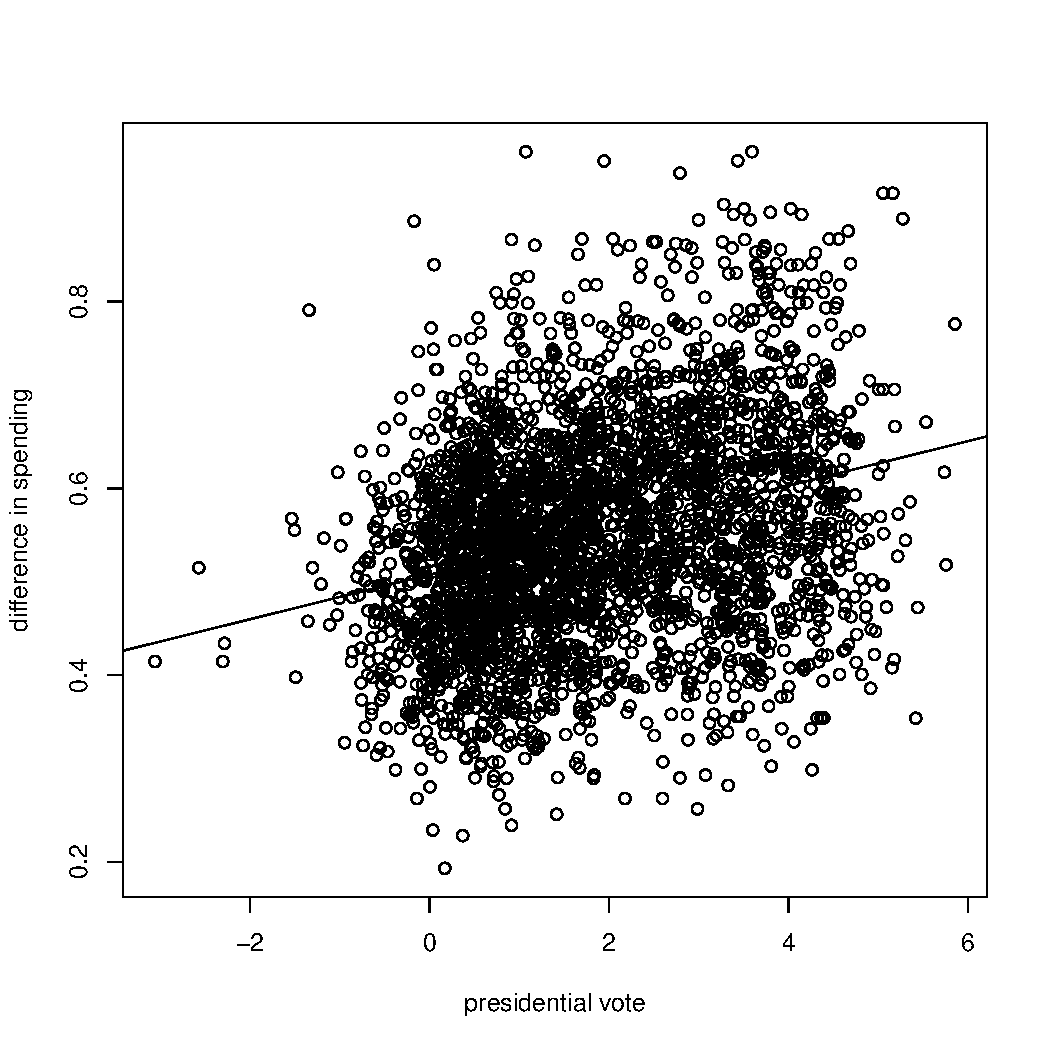
\includegraphics[width=.75\textwidth]{plot2.pdf}
		\end{figure}
		\vspace{.25cm}
		\item Save the residuals of the model in a separate object.	\lstinputlisting[language=R, firstline=59, lastline=60]{PS3_answer.R}
		\item Write the prediction equation.
		\lstinputlisting[language=R, firstline=63, lastline=64]{PS3_answer.R}
		The prediction equation is $\hat{Y_{i}}=0.507+0.024*X_i$.\\
	\end{enumerate}
	
	\newpage	
\section*{Question 3 (20 points)}

\noindent We are interested in knowing how the vote share of the presidential candidate of the incumbent's party is associated with the incumbent's electoral success.
	\vspace{.25cm}
	\begin{enumerate}
		\item Run a regression where the outcome variable is \texttt{voteshare} and the explanatory variable is \texttt{presvote}.\\
		I run the regression with X variable as \texttt{presvote} and Y variable as \texttt{voteshare}. I then check the estimateed coefficients of the model using \texttt{summary()}.\\
		\lstinputlisting[language=R, firstline=74, lastline=77]{PS3_answer.R}
		\begin{footnotesize}
			\begin{verbatim}
				Coefficients:
				Estimate Std. Error t value Pr(>|t|)    
				(Intercept) 0.441330   0.007599   58.08   <2e-16 ***
				presvote    0.388018   0.013493   28.76   <2e-16 ***
				---
				Signif. codes:  0 ‘***’ 0.001 ‘**’ 0.01 ‘*’ 0.05 ‘.’ 0.1 ‘ ’ 1
				
				Residual standard error: 0.08815 on 3191 degrees of freedom
				Multiple R-squared:  0.2058,	Adjusted R-squared:  0.2056 
				F-statistic:   827 on 1 and 3191 DF,  p-value: < 2.2e-16
				\end{verbatim}
			\end{footnotesize}
			
		\item Make a scatterplot of the two variables and add the regression line. 
			\begin{figure}[h!]\centering
				\caption{\footnotesize Scatterplot of \texttt{presvote} and \texttt{voteshare}.
				}\vspace{-1cm}
				\label{fig:plot3}
				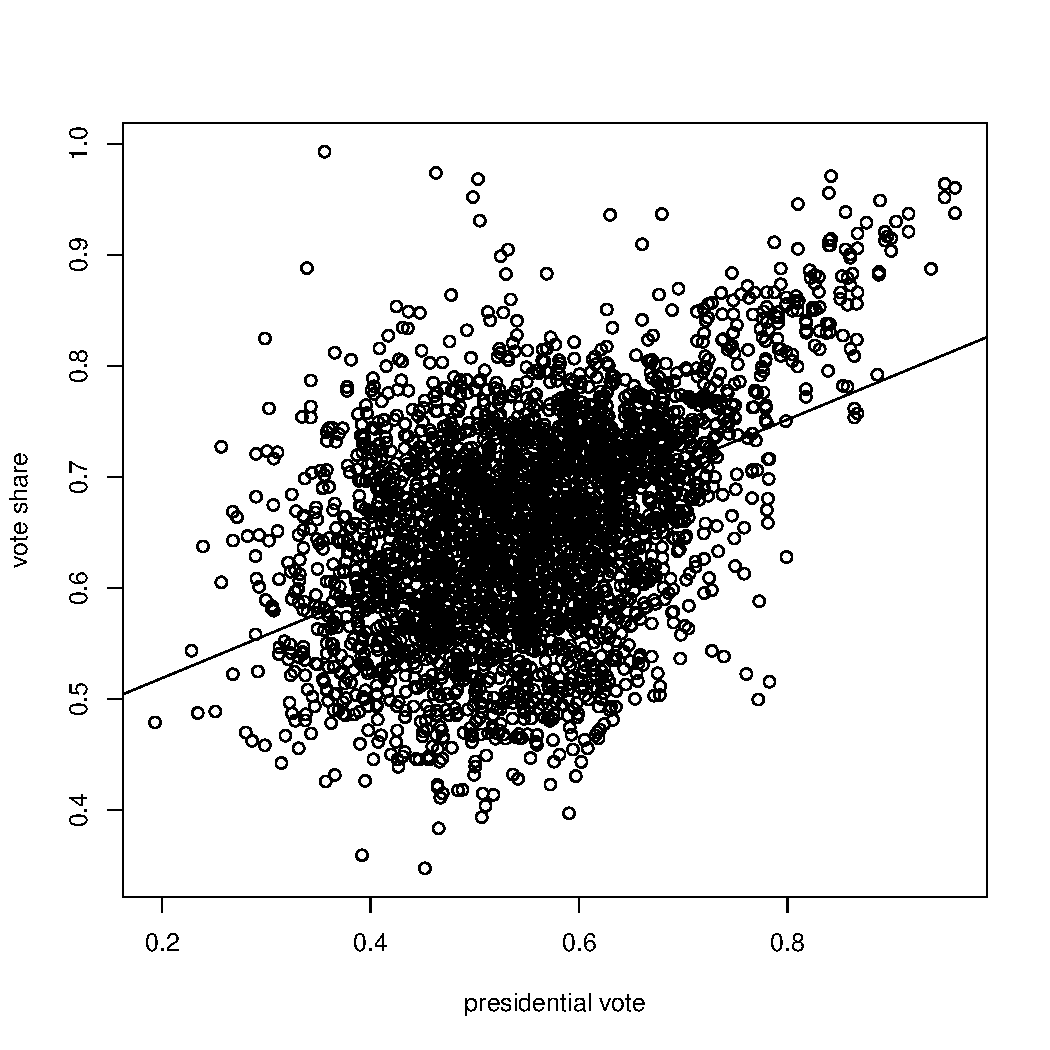
\includegraphics[width=.75\textwidth]{plot3.pdf}
			\end{figure}
			\vspace{.25cm}
		\item Write the prediction equation.\\
		\lstinputlisting[language=R, firstline=87, lastline=88]{PS3_answer.R}
		The prediction equation is $\hat{Y_{i}}=0.441+0.388*X_i$.\\
	\end{enumerate}
	

\newpage	
\section*{Question 4 (20 points)}
\noindent The residuals from part (a) tell us how much of the variation in \texttt{voteshare} is $not$ explained by the difference in spending between incumbent and challenger. The residuals in part (b) tell us how much of the variation in \texttt{presvote} is $not$ explained by the difference in spending between incumbent and challenger in the district.
	\begin{enumerate}
		\item Run a regression where the outcome variable is the residuals from Question 1 and the explanatory variable is the residuals from Question 2.\\
		I run the regression with X variable as \texttt{residuals2} and Y variable as \texttt{residuals1}. I then check the estimateed coefficients of the model using \texttt{summary()}.\\
		\lstinputlisting[language=R, firstline=98, lastline=101]{PS3_answer.R}
		\begin{footnotesize}
			\begin{verbatim}
			Coefficients:
			Estimate Std. Error t value Pr(>|t|)    
			(Intercept) -4.860e-18  1.299e-03    0.00        1    
			residuals_2  2.569e-01  1.176e-02   21.84   <2e-16 ***
			---
			Signif. codes:  0 ‘***’ 0.001 ‘**’ 0.01 ‘*’ 0.05 ‘.’ 0.1 ‘ ’ 1
			
			Residual standard error: 0.07338 on 3191 degrees of freedom
			Multiple R-squared:   0.13,	Adjusted R-squared:  0.1298 
			F-statistic:   477 on 1 and 3191 DF,  p-value: < 2.2e-16
			\end{verbatim}
		\end{footnotesize}
		\item Make a scatterplot of the two residuals and add the regression line. 
		\begin{figure}[h!]\centering
			\caption{\footnotesize Scatterplot of \texttt{residuals2} and \texttt{residuals1}.
			}\vspace{-1cm}
			\label{fig:plot4}
			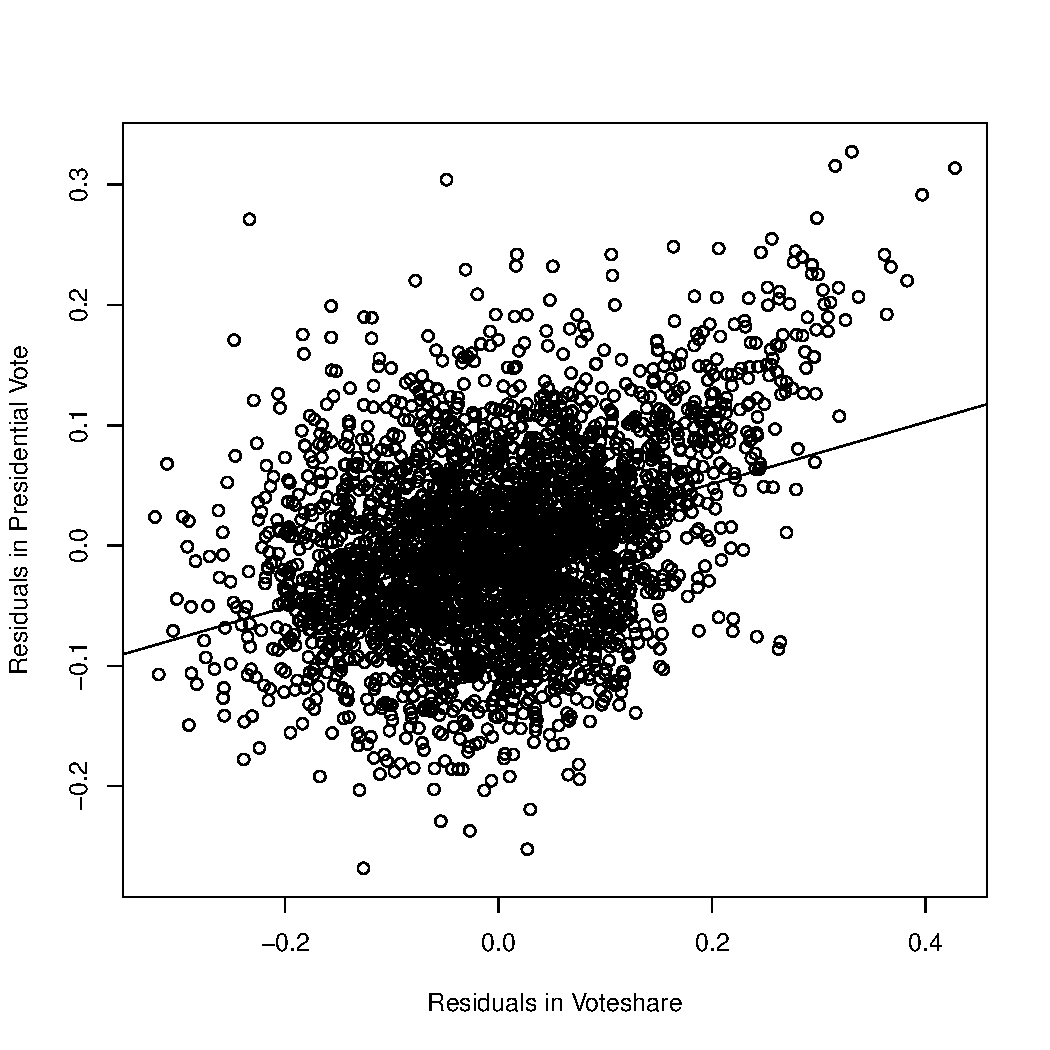
\includegraphics[width=.75\textwidth]{plot4.pdf}
		\end{figure}
		\vspace{.25cm}
		\item Write the prediction equation.
		\lstinputlisting[language=R, firstline=110, lastline=111]{PS3_answer.R}
		The prediction equation is $\hat{Y_{i}}=-4.860+0.256*X_i$.\\
	\end{enumerate}
	
	\newpage	

\section*{Question 5 (20 points)}
\noindent What if the incumbent's vote share is affected by both the president's popularity and the difference in spending between incumbent and challenger? 
	\begin{enumerate}
		\item Run a regression where the outcome variable is the incumbent's \texttt{voteshare} and the explanatory variables are \texttt{difflog} and \texttt{presvote}.\\	
		I run the regression with X variable as \texttt{difflog} and \texttt{presvote} and Y variable as \texttt{voteshare}. I then check the estimateed coefficients of the model using \texttt{summary()}.\\
		\lstinputlisting[language=R, firstline=122, lastline=125]{PS3_answer.R}  	
		\begin{footnotesize}
			
			\begin{verbatim}
			Coefficients:
			Estimate Std. Error t value Pr(>|t|)    
			(Intercept) 0.4486442  0.0063297   70.88   <2e-16 ***
			difflog     0.0355431  0.0009455   37.59   <2e-16 ***
			presvote    0.2568770  0.0117637   21.84   <2e-16 ***
			---
			Signif. codes:  0 ‘***’ 0.001 ‘**’ 0.01 ‘*’ 0.05 ‘.’ 0.1 ‘ ’ 1
			
			Residual standard error: 0.07339 on 3190 degrees of freedom
			Multiple R-squared:  0.4496,	Adjusted R-squared:  0.4493 
			F-statistic:  1303 on 2 and 3190 DF,  p-value: < 2.2e-16
			\end{verbatim}
		\end{footnotesize}
	\vspace{.25cm}
	\item Write the prediction equation.\\
	\lstinputlisting[language=R, firstline=128, lastline=129]{PS3_answer.R}
	The prediction equation is $\hat{Y_{i}}=0.4486+0.0355*X_(difflog)+0.2569*X_(presvote)$.\\
		\item What is it in this output that is identical to the output in Question 4? Why do you think this is the case?\\
	%	\item Reflect on your finding. Don't write anything. Just think about it.
	The coefficient of variable \texttt{presvote} is identical to the coefficient of \texttt{residual2}. It makes sense because \texttt{residual2} means how much of the variation in \texttt{presvote} is not explained by the model. 
	\end{enumerate}




\end{document}
